\documentclass{article}
\usepackage[utf8]{inputenc}
\usepackage{custom}

\title{LINMA 2120 - Seminars in Applied Mathematics \\
        High dimensional time-series prediction with missing values}
\author{Quentin Lété}
\date{December 4th, 2017}

\begin{document}

\maketitle

\section{Introduction}
What will the weather be like tomorrow ?
Will the price of oil drop in the coming weeks ?
How will the electricity consumption evolve in a particular neighborhood ?
People ask themselves such questions everyday.
What they have in common is that they all try to predict the value of a quantity that changes with the time.
With the increasing computational power provided by modern computers, people have been discovering more and more the value of data and the huge benefit that they can provide in many domains.
In a lot of applications, this data vary with time.
This is the case for the notions of price, consumption and production that are central to every market.
But this can be also the case for physical phenomenon, like the weather.
Time series analysis is the field that studies processes involving this kind of data. \\
In this work, we will give an overview of methods used to make predictions about time series.
We will particularly focus on methods that can recover missing values and that can deal with large-scale data.\\

This report will be organised as follows :
\begin{itemize}
\item Section \ref{prem} will give the main definitions and notations used in the rest of the report.
\item Section \ref{clas} will present the classical methods used in time-series modelling, i.e. autoregressive models and dynamic linear models.
\item Section \ref{sec:trmf} will develop the Temporal Regularized Matrix Factorization method proposed by Yu et al. (\cite{TRMF}).
\item Section \ref{over} will give an overview of the papers that cite \cite{TRMF}.
\item Section \ref{app} will develop a particular application of time series forecasting in more details.
\item Section \ref{dl} will develop another class of methods popular for prediction : deep learning methods.
\item Section \ref{conc} will give the final comments of the report.
\end{itemize}

\section{Preliminaries}
\label{prem}
Let us first give a definition of time series to explain the formal context in which we work. \\

\theoremstyle{definition}
\begin{definition}{Time series}
A time series is a sequence of data indexed by the time.
\end{definition}

A time series is thus a realization of a stochastic process which can be seen as a family of random variables indexed by the time. \\

We also define here a property of a stochastic process that will be useful later : the Markov property. \\

\theoremstyle{definition}
\begin{definition}{Markov property}
We say that $(Y_t)_{t \ge 0}$ is a Markov chain if for all $t > 0$
$$\pi(Y_t|Y_{1:t-1}) = \pi(Y_t|Y_{t-1})$$
where $\pi$ is the probability.
\end{definition}

This means that all the information about the past is completely carried out in the $Y_t$ at each step. With Markov chains, the joint distribution of observations take a fairly simple form :

$$\pi(Y_{1:t}) = \pi(Y_1) \cdot \prod_{j=2}^2 \pi(Y_j|Y_{j-1})$$

\subsection*{Notation}

Time series can be multidimentional, i.e. be a vector of several quantities that evolve with time. In that case, every such quantities are called streams. In this work, we will denote time series as matrices for which each line correspond to a stream and each column to the measurements at a fixed time. For instance, we could have a time series $Y \in \mathbb{R}^{n \times T}$. In this case, the columns of $Y$ will be noted in lowercase and bold form indexed on the time $t$, i.e. $\mathbf{y}_t$. The $i$-th row of $Y$ will be noted $Y_{i:}$ and correspond to the $i$-th stream.

\subsection*{Imputation vs Interpolation}

There are two ways of using the data provided to make inference on another value of the time series.
\begin{definition}{Imputation}
is using only the values of a fixed time to make predictions on another value of this particular time.
\end{definition}

\begin{definition}{Interpolation}
 is using the data of a single stream to infer on another value of this stream.
\end{definition}

\section{Classical methods}
\label{clas}
In this section, we present classical methods used for time series forecasting.
These classical methods include AR (autoregressive) models and DLM (dynamic linear models) and are used for prediction.
Let us explain sequentially these models.

\subsection*{Autoregressive models}
As explained in \cite{pmlr-v37-anava15}, the idea of this model is to represent each observation as a noisy linear combination of previous observations.
Formally, let $\mathcal{L}$ be the set of time indices that encodes the dependence between the observations over time. If $\mathbf{x}_t \in \mathbb{R}^k$ is the measurement at time $t$ and if the lag $|\mathcal{L}| = p$, the AR(p) model prametrized by the coefficient matrix $\mathcal{W} = \{W^{(l)} \in \mathbb{R}^{k \times k} : l \in \mathcal{L} \}$ can be written as

\begin{equation}
\mathbf{x}_t = \sum_{l \in \mathcal{L}} W^{(l)} \mathbf{x}_{t-l} + \epsilon_t
\label{eq:ar}
\end{equation}

where $\{ \epsilon_t \}_{t \in \mathbb{Z}}$ is a Gaussian noise vector. For simplicity, we will suppose that $\epsilon_t \sim \mathcal{N}(0, \sigma^2 I_k)$.

This moedel is motivated by a theorem due to Wold that states that a stationary process can be represented by a MA($\infty$) model, that is

$$\mathbf{x}_t = \sum_{i=1}^{\infty} \beta_i \epsilon_{t-i} + \epsilon_t$$

where $\sum_{i=1}^\infty \beta_i < \infty$ and where MA stands for Moving Average. And if $\{ \mathbf{x}_t \}_t^\infty$ is invertible, we also have that it can be represented by an AR$(\infty)$ model, that is

$$\mathbf{x}_t = \sum_{i=1}^{\infty} \alpha_i \mathbf{x}_{t-i} + \epsilon_t$$

With this theorem, it seems natural to use AR$(p)$ models for prediction. \\

Another popular model in this class is the ARMA (Autoregressive Moving Average) model that is simply a combination of the two previous ones. It can be written as

$$\mathbf{x}_t + \sum_{l \in \mathcal{L}} W^{(l)} \mathbf{x}_{t-l} = \sum_{i=1}^{K} \alpha_i \mathbf{x}_{t-i} + \epsilon_t$$

This in turn is the basis for more complicated models like ARMAX that accounts for exogeneous input or ARIMA that extends ARMA to deal with non-stationary processes.

\subsection*{Dynamic Linear Models}
DLM is a simpler model of a more general framework called state space models \cite{DLMR}. \\

\begin{definition}{State space model}
A state space model consist of two time series : a $\mathbb{R}^p$-valued time series $\{\mathbf{x}_t\}$ and a a $\mathbb{R}^m$-valued time series $\{\mathbf{y}_t\}$ satisfying the following assumptions :

\begin{itemize}
        \item ($\mathbf{x}_t$) is a Markov chain
        \item Conditionnaly on $(\mathbf{x}_t)$, the $\mathbf{y}_t$'s are independent and the $\mathbf{y}_t$'s depends only on $(\mathbf{x}_t)$
\end{itemize}
\label{statespace}
\end{definition}

The idea behind this model is that the seris $\mathbf{y}_t$ is determined by a latent process $\mathbf{x}_t$. The $\mathbf{x}_t$'s usually represent all the observable physical variables that have an influence on the variable of interest. For instance, if we try to predict the price of electricity in the future, the latent variables could be the temperature, the wind speed, the sunshine, ... Note that this ($\mathbf{x}_t$) is assumed to be a Markov chain. \\

In general, a state space model consists in two equations : an \textbf{obvservation equation} which gives $\mathbf{y}_t$ in function of $\mathbf{x}_t$ at each step and an \textbf{evolution equation} which gives $\mathbf{x}_t$ in function of $\mathbf{x}_{t-1}$. Both equations are pertubed by noise. This can be written as

$$\mathbf{y}_t = f_t(\mathbf{x}_t, v_t)$$
$$\mathbf{x}_t = g_t(\mathbf{x}_{t-1}, w_t)$$

To be complete we also have to specify the prior distribution for $\mathbf{x}_0$. \\

With that general state space model defined, it is possible to define the DLM which is a special case of it with linear functions and Gaussian noise. \\

\theoremstyle{definition}
\begin{definition}{DLM}
A dynamic linear model (DLM) is specified by a Normal prior distribution for the p-dimensional state vector at time t = 0,
$$\mathbf{x}_0 \sim \mathcal{N}_p(m_0, C_0)$$
together with a pair of equations for each time $t \ge 1$,

$$\mathbf{y}_t = F_t\mathbf{x}_t + v_t, \hspace{3cm} v_t \sim \mathcal{N}_m(0, V_t)$$
$$\mathbf{x}_t = G_t\mathbf{x}_{t-1} + w_t, \hspace{3cm} v_t \sim \mathcal{N}_p(0, W_t)$$

where $F_t$ and $G_t$ are known matrices of order $m \times p$ and $p \times p$ respectively.
\end{definition}

\subsubsection*{Forecasting}

Based on this model, how can we predict the future observation ? The problem is solved by use of the \textbf{Kalman filter}. This filter is based on the idea that, due to the markovian property of the state vector and the assumption of conditional independence of the observations, the density of the state and the observation knowing their previous values can be computed recursively. Moreover, because the equations are linear and the noise and prior distribution are Gaussian, it is possible to prove that the random vector $(\mathbf{x}_0, ..., \mathbf{x}_t, \mathbf{y}_0, ..., \mathbf{y}_t)$ follows a mutlivariate Gaussian distribution. Therefore, only the mean and covariance matrix has to be computed. The Kalman filter gives the recursion equation for them : \\

\begin{theorem}
Let $\mathcal{D}_t$ be the information provided by the first $t$ observations $\mathbf{y}_1, ..., \mathbf{y}_t$.
Then, if
$$\mathbf{x}_{t-1} \sim \mathcal{N}(m_{t-1}, C_{t-1}),$$
where $t \ge 1$, then

\begin{enumerate}[(a)]

\item the one-step-ahead predictive density of $\mathbf{x}_t$ given $\mathcal{D}_{t-1}$ is Gaussian with parameters

$$a_t = E(\mathbf{x}_t|\mathcal{D}_{t-1}) = G_tm_{t-1}$$
$$R_t = \text{Var}(\mathbf{x}_t|\mathcal{D}_{t-1}) = G_tC_{t-1}G_t' + W_t$$

\item the one-step-ahead predictive density of $Y_t$ given $\mathcal{D}_{t-1}$ is Gaussian with parameters

$$f_t = E(\mathbf{y}_t|\mathcal{D}_{t-1}) = F_ta_t$$
$$Q_t = \text{Var}(\mathbf{y}_t|\mathcal{D}_{t-1}) = F_tR_tF_t' + V_t$$

\item the filtering density of $\mathbf{x}_t$ given $\mathcal{D}_t$ is Gaussian with parameters

$$m_t = E(\mathbf{x}_t|\mathcal{D}_{t}) = a_t + R_tF_t'Q_t^{-1}e_t$$
$$C_t = \text{Var}(\mathbf{x}_t|\mathcal{D}_{t}) = R_t - R_tF_t'Q_t^{-1}F_tR_t$$

where $e_t = \mathbf{y}_t-f_t$ is the forecast error.

\end{enumerate}

\end{theorem}

This theorem gives us everything we need to predict the behaviour of the observations for a time series modeled by a DLM. \\

It can be seen that the complexity of this algorithm is $\mathcal{O}(kn^2T + k^3T)$.
This rather high complexity can become prohibitive when dealing with high-dimensional data. For instance, it is noted in \cite{TRMF} that using a common package in $R$ for DLM, problems with $n \ge 32$ cannot be solved. \\

Another problem with the two classical methods that we have described is that it is not clear how missing data would be dealed with. Yet, missing data are common in many application involving time series and can be due to occlusions or misfunction of sensor, among others. \\

We will now present the novel approach to make predictions about high-dimensional time series published in \cite{TRMF}.

\section{Temporal Regularized Matrix Factorization}
\label{sec:trmf}

\subsection*{Framework}
The authors place themselves in a framework similar to the state space model defined in definition \ref{statespace}.
The difference is that here $\mathbf{x}$ is not supposed to respect the Markov property. Moreover, the observation equation is assumed to be linear.
Formally, this can be described by the following equations :

\begin{equation}
\mathbf{y}_t = F\mathbf{x}_t + \eta_t
\end{equation}
\begin{equation}
\mathbf{x}_t = M_{\Theta}(\{\mathbf{x}_{t-l} : l \in \mathcal{L} \}) + \epsilon_t
\label{eq:evol}
\end{equation}

The vector noise $\eta_t$ and $\epsilon_t$ are supposed to be Gaussian. These equations are parametrized by two sets : $\mathcal{L}$ that contains the number of previous state vectors on wich $\mathbf{x}_t$ depends and $\Theta$ that contains the weights associated to each vector in time.

\subsection*{Matrix factorization formulation}
The primary obsevation made by the authors is that when we stack all $\mathbf{x}_t$ in a matrix $X$ and if we do the same with the $\mathbf{y}_t$ in the matrix $Y$, we can see that $Y \approx FX$. Of course, noise has been omitted in this equation and this is why it is not an equality. We notice that this idea enables to do at the same time interpolation and imputation, as defined above. \\

With this observation, our problem becomes a problem of matrix factorization which has been widely studied in the past. For instance, this is a key element in some recommender systems and the use of matrix factorization in this context to perform machine learning has been used during the Netflix prize in 2007.
In the context of the Netflix prize, the incomplete matrix of ratings was decomposed into a matrix for the users and a matrix for the items. Those two matrices were learned by minimizing a mean square error on the data. \\

A similar approach can be used in our context. If we denote by $\mathbf{f}_i^\top$ the i$^\text{th}$ row of the matrix F and by $\Omega$ the set of observed entries, we could learn the $X$ and $F$ factors as

\begin{equation}
\underset{F,X}{\text{min}} \sum_{(i,t) \in \Omega} (Y_{it} - \mathbf{f}_i^\top\mathbf{x}_t)^2 + \lambda_f \mathcal{R}_f(F) + \lambda_x \mathcal{R}_x(X)
\label{eq:model}
\end{equation}

where $\mathcal{R}_f(F)$ and $\mathcal{R}_x(X)$ are regularization factors on $F$ and $X$ respectively. These factors are important to prevent overfitting and to take into accounts possible dependecies between the different entries of the matrices. \\
The link that has just been established between the general framework and matrix factorization approaches is important but it still does not tell us how to use equation \ref{eq:evol} to account for the temporal dependencies. We also need to describe how forecasting could take place in this framework. \\
In classical MF applications like the one mentionned earlier for recommender systems, the regularization factors are often taken as the norm of the matrix (for example the Frobenius norm) to penalize high values of the larned elements. However, here, this choice would not be a good idea as it would not take into account the temporal dependecies that naturally exists in the $\mathbf{x}_t$s. In \cite{TRMF}, the authors propose a choice of regularization factor which remedies that problem.

\subsection*{Temporal regularization}

The goal in this section is to describe a choice of regulization factor that is called $\mathcal{T}_M(X | \Theta)$ that will promote the relationship between the $\mathbf{x}_t$s given in (\ref{eq:evol}).
Recall that $\Theta$ in our model contains the information that links the $\mathbf{x}_t$s together. The idea proposed is to take the log-likelihood of the $\mathbf{x}_t$s knowing $\Theta$. This is formalized by the following equation :

$$\mathcal{T}_M(X | \Theta) = -\log{\mathbb{P}(\mathbf{x}_1, ..., \mathbf{x}_T|\Theta)}$$

It can be seen that the lower this factor is, the more plausible it is to observe this set of $\mathbf{x}_t$s according to (\ref{eq:evol}). Note that the logarithm in this equation is there for computational reasons only. If $\Theta$ is given, then we can use directly $\mathcal{T}_M(X | \Theta)$ as the regularization factor for $X$. When it is not given, a regularization for $\Theta$ should be added to \ref{eq:model} which becomes

\begin{equation}
\underset{F,X,\Theta}{\text{min}} \sum_{(i,t) \in \Omega} (Y_{it} - \mathbf{f}_i^\top\mathbf{x}_t)^2 + \lambda_f \mathcal{R}_f(F) + \lambda_x \mathcal{T}_M(X | \Theta) + \lambda_{\theta} R_{\theta}(\Theta)
\label{eq:model_theta}
\end{equation}

It is important to note that with this formulation, $\Theta$ can thus be learned from the data like $F$ and $X$. This is another important avantage that TRMF has compared to other approaches like graph-based regularization.
Once $\Theta$ is learned, we can use it in our model and use equation (\ref{eq:evol}) to predict that next latent vector $\mathbf{x}_t$, which can in turn be used to predict $\mathbf{y}_t$ as $F\mathbf{x}_t$. \\
Another feature that was missing from the classical method was the possibility to deal missing entries. With the TRMF technique, we can simply estimate the missing entries of $Y$ as $Y_{it} = \mathbf{f}_i^\top\mathbf{x}_t$.
This is one big advantage of matrix factirization and it is central to many of its application like recommender systems. \\
Finally, the MF framework can also be used to perform clustering. Again, this is similar to what has already been proposed in classical use of MF. The $\mathbf{f}_i$ vector can be interpreted as the latent embedding factor of the $i^\text{th}$ time series in $Y$ and thus clusering algorithms can directly be applied to these vectors.

\subsubsection*{Extensions}
This general TRMF framework can be conveniently extended to account for different aplications dependent extensions. In this section, we prensent $3$ useful ones.

\paragraph{Known fetures}
In the classical machine leaning framework, every item is associated with a time invariant feature vector. In the study of time series, it is common that in addition to the time dependent data, some known features are available on the objects and it is important to be able to incorporate them in the model to improve performances. Our TRMF framework can be easily extended to account for this additional feature vector for item $i$ denoted $\mathbf{a}_i$ as follows :

\begin{equation}
\underset{F,X,\Theta}{\text{min}} \sum_{(i,t) \in \Omega} (Y_{it} - \mathbf{a}_i^\top F \mathbf{x}_t)^2 + \lambda_f \mathcal{R}_f(F) + \lambda_x \mathcal{T}_M(X | \Theta) + \lambda_{\theta} R_{\theta}(\Theta)
\label{eq:model_feature}
\end{equation}

This formulation has two main advantages :
\begin{itemize}
\item A new time series $Y_{i't}$ can know be estimated without knowledge of any additional observation up to time $T$. We can simply and directily estimate it as $Y_{i't} = \mathbf{a}_i'^\top F \mathbf{x}_t$ if the feature vector is available
\item If $\mathbf{a}_i \in \mathbb{R}^d$, this has also the effect of reducing the dimensions of $F$ from $n \times k$ to $d \times k$ which can improve the efiiciency of the algorithm.
\end{itemize}

\paragraph{Graph information among time series}
Sometimes, a graph based information is available on the time series. This graph encodes relationships between them. The goal is to define a regularization on $F$ that will tend to promote the structure defined by the graph.
Given a graph $G$ on the time series with weights $G_{ij}$ on the edge $i-j$, we can take the following graph regularization factor :
$$\mathcal{G}(F|G,\eta) = \frac{1}{2}\sum_{i\sim j}G_{ij}\|\mathbf{f}_i - \mathbf{f}_j\|^2 + \frac{\eta}{2}\sum_i \|\mathbf{f}_i\|^2$$

Our problem then becomes simply :

\begin{equation}
\underset{F,X,\Theta}{\text{min}} \sum_{(i,t) \in \Omega} (Y_{it} - \mathbf{f}_i^\top\mathbf{x}_t)^2 + \lambda_f \mathcal{G}(F|G,\eta) + \lambda_x \mathcal{T}_M(X | \Theta) + \lambda_{\theta} R_{\theta}(\Theta)
\label{eq:model_graph}
\end{equation}

\paragraph{Temporal-regularized tensor factorization}
It is also possible to extend our framework to tensor factorization with evolution over time. To take again the example of movie recommender system, it is sometimes useful to model the variation over time of the preferences of a user or to model some kind of fashion effect associated to a movie. In the classial MF framework, we thus incorporate time labelled data. If $P$ denotes the matrix of latent enbeddings of the users and $Q$ of the movies, our model can be extended as :

\begin{equation}
\underset{P,Q,X,\Theta}{\text{min}} \sum_{(i,j,t) \in \Omega} (Y_{ijt} - \langle \mathbf{p}_i,\mathbf{q}_j,\mathbf{x}_t \rangle )^2 + \lambda_p \mathcal{R}_p(P) + \lambda_q \mathcal{R}_q(Q) + \lambda_x \mathcal{T}_M(X | \Theta) + \lambda_{\theta} R_{\theta}(\Theta)
\label{eq:model_tensor}
\end{equation}

where $\langle \mathbf{p}_i,\mathbf{q}_j,\mathbf{x}_t \rangle$ is defined as $\sum_r p_{ir}q_{jr}x_{tr}$

\subsection*{Autoregressive Temporal Regularization}
TRMF have been described until here using a very general evolution equation (\ref{eq:evol}). In this section, we will apply the TRMF framework on a autoregressive model for the latent embeddings. Let us recall equation (\ref{eq:ar}) which defines the AR model for the time series $\mathbf{x}_t$ parametrized by the lag set $\mathcal{L}$ and the weights $W^{(l)}$ :
$$\mathbf{x}_t = \sum_{l \in \mathcal{L}} W^{(l)} \mathbf{x}_{t-l} + \epsilon_t$$

We would like to define a regularization factor on $X$ that promotes this model for the $\mathbf{x}_t$. A natural choice would be the following :

\begin{equation}
\mathcal{T}_{AR}(X|\mathcal{L}, \mathcal{W}, \eta) = \frac{1}{2} \sum_{t=m}^T \norm{\mathbf{x}_t - \sum_{l \in \mathcal{L}} W^{(l)} \mathbf{x}_{t-l}}^2 + \frac{\eta}{2} \sum_t \|\mathbf{x}_t\|^2
\label{eq:tar}
\end{equation}

where $m := 1+\text{max}(\mathcal{L})$ and the last term has been added to ensure strong convexity. \\


As explained previously, the TRMF framework allows us to learn the weight matrices $W^{(l)}$ when they are not known. However, as $W^{(l)} \in \mathbb{R}^{k \times k}$, the number of weights to be learned would be $|\mathcal{L}|k^2$ which can be large and lead to overfitting. We could reduce the amount of weights by assuming that the $W^{(l)}$ are diagonal. This reduces the number of weights to $|\mathcal{L}|k$.
This correseponds to assuming that each element of the observation vector $\mathbf{y}_t$ is only influenced by the corresponding elements in the observations $\{\mathbf{y}_{t-l}\}_{l \in \mathcal{L}}$ \\
This has the effect of decoupling each time series from each other (when we talk about each time series, we mean each line of the $X$ or the $Y$ matrices). Let us rewrite $\mathcal{T}_{AR}$ in a way that enhances this decoupled structure. \\
Let us denote $\mathcal{W}$ as the $k \times L$ matrix where the $l$-th column in the diagonal of $W^{(l)}$ and note that for $l \notin \mathcal{L}$, the $l$-th column of $\mathcal{W}$ is a zero vector.
Let $\bar{\mathbf{x}}_r^{\top} = [..., X_{rt}, ...]$ be the $r$-th row of $X$ and $\bar{\mathbf{w}}_r^{\top} = [..., \mathcal{W}_{rl}, ...]$ be the $r$-th row of $\mathcal{W}$. Then, equation (\ref{eq:tar}) can be written as


$$\mathcal{T}_{AR}(X|\mathcal{L}, \mathcal{W}, \eta) = \sum_{r=1}^k \mathcal{T}_{AR}(\bar{\mathbf{x}}_r|\mathcal{L}, \bar{\mathbf{w}}_r, \eta)$$
$$\mathcal{T}_{AR}(\bar{\mathbf{x}}_r|\mathcal{L}, \bar{\mathbf{w}}_r, \eta) = \frac{1}{2} \sum_{t=m}^T \Big(x_t - \sum_{l \in \mathcal{L}} w_l x_{t-l} \Big)^2 + \frac{\eta}{2} \|\bar{\mathbf{x}}_r\|^2$$

Let us also note that when $L = 1$, we have exactly the Dynamic Linear Model with a general weight matrix $W^{(1)}$.

\subsubsection*{Optimizing TRMF with AR Temporal Regularization}
Using $\mathcal{T}_{AR}$ as the regularization factor for $X$ in equation (\ref{eq:model_theta}), we get the following optimization problem :

\begin{equation}
\underset{F,X,\Theta}{\text{min}} \sum_{(i,t) \in \Omega} (Y_{it} - \mathbf{f}_i^\top\mathbf{x}_t)^2 + \lambda_f \mathcal{R}_f(F) + \lambda_x \sum_{r=1}^k \mathcal{T}_{AR}(\bar{\mathbf{x}}_r|\mathcal{L}, \bar{\mathbf{w}}_r, \eta) + \lambda_{w} R_{w}(\mathcal{W})
\label{eq:model_ar}
\end{equation}

The authors in \cite{TRMF} propose to solve (\ref{eq:model_ar}) with alternating minimization. Therefore, the minimization of the parameters when the others are fixed reduces to well-known methods.

\subsection*{Conclusion}
In this section, we have presented a new method to deal with time varying data, i.e. Temporal Regularized Matrix Factorization. As its name indicates, this method is based on Matrix Factorization techniques and makes use of a particular regularization factor to account for temporal dependencies between the data. \\
The general framewok was first discussed. Then, the method was specified in the case of an $AR$ process for the latent embedding. \\
The main advantages of TRMF is that it is able to deal with missing data by estimating them with the latent embeddings provided by Matrix Factorization. This method has also the advantage of being more scalable than classical methods. Finally, with the framework described, the exact equation for the latent vector $\mathbf{x}_t$ must not be known \emph{a priori}.

\section{Overview of related research}
\label{over}
In this section, we will have a look at other ongoing research ideas that are linked to TRMF by giving an overview of the papers that cite \cite{TRMF}. Some of these topics will be explained in more details in the next sections. In particular, section \ref{app} will develop the idea of using MF to make prediction on electrical quantities. Section \ref{dl} will detail the use of deep learning in this context and evoke in particular two different network architectures. \\

In \cite{1bit}, the authors explore the problem of recovering entries in a dynamically changing low-rank matrix with known factorization and one-bit obsevation on those entries. A one-bit LOWEMS (Locally Weighted Matrix Smoothing) is formulated. The idea of LOWEMS but this time for recovery with linear measurements is also explored in \cite{LOWEMS}.\\
\cite{linear1} and \cite{linear2} extend Nonnegative Matrix Factorization (NMF) to take into account linear measurements instead of matrix entries. The work is motivated by electricity consumption prediction. \\
A few recent papers have also taken deep learning approaches to deal with the time-varying property of the data. This is the case of \cite{ChungGCB14}, \cite{Yoon2017MultidirectionalRN}, \cite{deep1} and \cite{deep2}. \\
Matrix Factorization is still used to model temporaal effects in recommender systems, like in \cite{rs1} and \cite{rs2}. \\
Finally, another ongoing part of research on this subject is focusing on linear state space model for time series forecasting (\cite{ss1}, \cite{ss2}). \\

\section{Application to electrical quantities forecasting}
\label{app}
As stated above, TRMF can be used in various contexts that include time varying data. One import sector that deals with this kind of data is the energy sector.
For instance, in electricity market modelling, it is tremendously important to be able to forecast the elctricity demand or the production of renewable energy to adapt the centralized production.
In \cite{Elec}, this idea of using TRMF to forecast electrical quantities is developed.
The framework used is similar to \cite{TRMF} while being a bit simpler. Matrix factorization is used to predict new values but the temporal regularization is ignored. The idea is that we have a dataset containing history of values of a certain electrical quantity. If we arrange this data in matrix form, future values can be predicted by minimizing the error of the matrix factorization on known entries, similarly to what was proposed for Matrix Factorization in the context of recommender systems. \\
To be slightly more formal, let us apply the idea on an example. We have data that corresponds to wind speed at each hour of the day from 1986 to 1995. We suppose that data of the year 1995 are missing and that we wish to recover or predict them. We build the matrix $Y$ as the matrix with $3652$ rows that correspond to the $3652$ days of the years $1986$ to $1995$ and $24$ columns at each hour in these days. The entry $Y_{i,t}$ is the wind speed that was recorded at hour $t$ of day $i$. If the wind speed for the last hour of the last day is missing, the matrix look like

$$Y = \begin{bmatrix} Y_{1,1} & \hdots & Y_{1,24} \\ \vdots & \ddots & \vdots \\ Y_{3652,1} & \hdots & ? \end{bmatrix}$$

Let $\Omega$ be the set of row-column pairs that have a known entry in the matrix $Y$. The matrices $F \in \mathbb{R}^{3652 \times k}$ and $X \in \mathbb{R}^{k \times 24}$, where $k$ is the length of the latent embedding and is a parameter of the method, are determined by the following optimization problem

$$\underset{F,X}{\text{min}} \sum_{(i,t) \in \Omega} \Big( Y_{i,t} - \mathbf{f}_i^{\top}\mathbf{x}_t \Big)^2 + \lambda (\|\mathbf{f}_i\|^2 + \|\mathbf{x}_t\|^2) $$

This optimization problem can be solved by stochastic gradient descent. Then, $?$ is estimated as $? \approx \mathbf{f}_{3652}^{\top}\mathbf{x}_{24}$ \\
It is shown in \cite{Elec} that this approach can yields better predictions than ARIMA (Autoregressive integrated moving average) models in certain situations. \\

It should be noted that the approach presented in \cite{Elec}, altough using the same idea as \cite{TRMF} of Matrix Factorization for time-series prediction, does not develop any Temporal Regulization technique that could improve the results. Except the idea of the application to electrical quantities forecasting, it does not provide new ideas compared to the basic framework of matrix factorization for prediction that was developed during the Netflix prize.

\section{Deep learning methods}
\label{dl}
Another class of methods designed to handle time varying data are methods based on deep learning.
Deep learning techniques construct what is called a Neural Network, i.e. a model inspired by the human brain to perform machine learning tasks. In its simplest form, it embeds a directed-graph structure composed of several layers of nodes (neurons) provided with thresholds and functions of activation (similarly to real neurons). Nodes are connected to each other by edges (axons) provided with weights. \\
Several people have designed Neural Networks to deal with times series prediction. In this section, we present two of such methods.

\subsection*{Multi-directional Recurrent Neural Networks}
This method is developed in \cite{Yoon2017MultidirectionalRN}.
We have seen that there are two ways of forecasting values in a time series.
The first one, called interpolation, uses only intra-stream data whereas the second one, called imputation uses only inter-stream data at a given time stamp.
Matrix Factorization has the important advantage to allow to do both at the same time.
Some people have tried to come up with other ideas to combine inter-stream and intra-stream information to make predictions. This is the case of the authors of \cite{Yoon2017MultidirectionalRN} where a deep learning approcach is taken. \\

\subsubsection*{Architecture}
The Neural Network designed is called a Multi-directional Recurrent Neural Network. Let us exmplain the particularities of such a network. In the following, we denote by $Y_{it}$ the element of the time serie that we want to estimate and we denote it's estimate by $\tilde{Y}_{it}$.

\paragraph{Recurrent} A Recurrent Neural Network is a network of neurons with feedback connections. In terms of the neurons graph, it means that the graph is allowed to contain loops. \\
More formally, this Neural Network architecture maintains a recurrent hidden state whose activation at each time is dependent on that of the previous time. If we have a input sequence $(x_1, ..., x_T)$, it updates the hidden state by

$$\mathbf{h}_t = g(W\mathbf{x}_t + U\mathbf{h}_{t-1})$$

where $g$ is an activation function (logistic sigmoid, hyperbolic tangent, ...) \cite{ChungGCB14}.

\paragraph{Multi-directional} This means that the network operate within streams and across streams. The network will contain two blocks : the interpolation block first that will operate within streams and then the imputation block. Moreover, the interpolation block is formed of Bi-directional Neural Networks. These networks have the property of being split into two sub-networks that are combined at the output. The inputs of the two sub-networks are respectively the sequence of data recorded before time $t$ $(Y_{i,1:t-1})$ and after time $t$ $(Y_{i,t+1:T})$. The authors of \cite{Yoon2017MultidirectionalRN} propose to respectively lag and advance the inputs in these two netwroks as represented on the folllowing figure :

\begin{figure}[H]
\centering
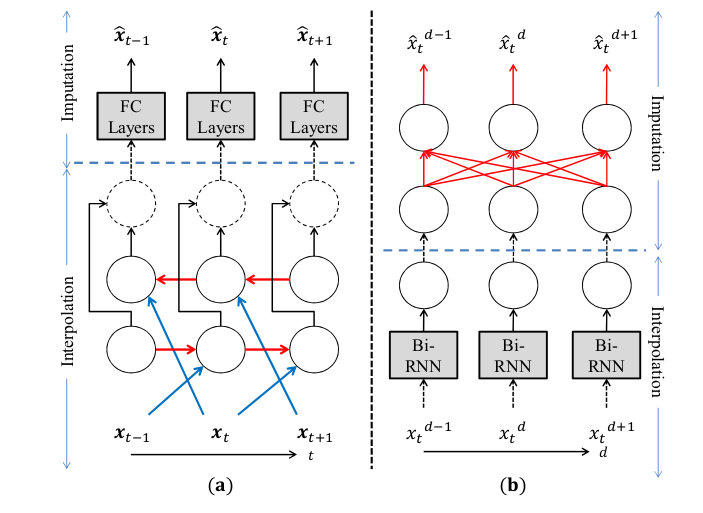
\includegraphics[scale=0.3]{MRNN}
\caption{Schematic representation of the architecture of the Multi-dimensional Neural Network from \cite{Yoon2017MultidirectionalRN}. (a) Time dimension, (b) Feature dimension.}
\label{im:MRNN}
\end{figure}

In figure \ref{im:MRNN}(a), we can see the Bi-directional sequences as first layer of the network aswell as the lag and advance performed in the input. In what concerns the feature dimension (imputation block), a fully connected (FC) network was used.

\subsubsection*{Learning}
As usual in Machine Learning, the training is done by minimizing an error. Here, the mean-squared error (MSE) is chosen. Consider that $\Omega$ contains the pairs of indices corresponding to the entries of $Y$ that we would like to estimate. Then, the MSE can be written as follows :

$$MSE(\Omega, Y, \tilde{Y}) = \frac{\sum_{(i,t) \in \Omega} (\tilde{Y}_{it} - Y_{it})^2}{|\Omega|}$$

It should be noted that, of course, we shouldn't une $Y_{it}$ when computing $\tilde{Y}_{it}$. This entry is supposed to be unknown and is hidden in the learning phase.

\subsubsection*{Results}
It is shown in an experimental part in \cite{Yoon2017MultidirectionalRN} that this method can yield better results than TRMF on some benchmark instances.

\subsection*{Traffic forecasting}
In \cite{Traffic}, Neural Networks are used in the context of spatiotemporal traffic forecasting. Traffic forecasting represent and interesting and challenging topic in time series forecasting as it requires to combine temporal and spatial information to make predictions. Moreover, such problems are usually large-scale problems and the inherent physical phenomenon that traffic represent is complex and highly nonlinear. \\
The authors of \cite{Traffic} propose to model the spatial dependency by a random-walk process on a graph to account for the diffusive nature of traffic and to model the temporal dynamics using a so-called Diffusion Convolutional Recurrent Neural Network. \\
More formally, we suppose that there are $N$ sensors located on the road network that measure a set $P$ of features related to the traffic at that point.
The sensor network is modeled as a directed weighted graph $\mathcal{G}(\mathcal{V}, \mathcal{E}, W)$ where $\mathcal{V}$ is the set of nodes with $|\mathcal{V}| = N$, $\mathcal{E}$ is the set of edges and $W$ is the weights matrix. At each time stamp, the $P$ features are recorded at every node. This is denoted by the matrix $Y^{(t)} \in \mathbb{R}(P \times N)$ that represents the values of the recorded features at time $t$.
The goal of traffic forecasting is, knowing the matrices $Y^{(t)}$ for $t \in [1,...,T]$ and the graph $\mathcal{G}$, to estimate the matrices $Y^{(t)}$ for $t \in [T+1, ..., T']$.

\subsubsection*{Spatial dependency}
As stated above, the spatial dependency is simply modeled by a random walk on the graph $\mathcal{G}$. The stationary ditribution of the random walk can be easily estimated. Indeed, let us denote by $\alpha$ the restart probability of the radom process. Then the stationary distribution $\mathcal{P} \in \mathbb{R}^{N \times N}$ can be computed as

$$\mathcal{P} = \sum_{k=0}^{\infty} \alpha (1-\alpha)^k (D_{O}^{-1}W)^k$$

where $D_{O} = \text{diag}(W\mathbf{1})$ and $\mathbf{1}$ is the vector of ones. Hence $(D_{O}^{-1}W)$ is the row normalised weight matrix. The $i$-th row of $\mathcal{P}$ represents the likelihood of diffusion from node $v_i \in \mathcal{V}$, hence the proximity with respect to the node $v_i$.

\subsubsection*{Temporal dynamics}
The temporal dynamics are modeled with a particuliar type of Neural Netork called Gated Recurrent Unit (GRU). As explained in \cite{ChungGCB14}, this is a slightly modified version of RNN to capture dependecies of different time scales. Without entering into too much details, the idea is simply to update the recurrent unit as a linear combination of the previous recurrent unit and the newly computed unit. \\
The particularity of \cite{Traffic} is that the weights of the GRU depends on the stationary distribution $\mathcal{P}$ making it a so-called Diffusion Convolutional Gated Recurrent Unit (DCGRU).

\section{Conclusion}
\label{conc}
Time series prediction is used in many application. The need for robust models that can deal with high-dimensional data makes it an active field of research. In this report, we first described the classical methods and highlighted their main limitations. Then, we explained the Temporal Regularized Matrix Factorization approach and showed how it can overcome the previously mentionned limitations. Then, we gave an overview of the recent ideas that are currently being proposed in this field and we detailed how MF can be applied to prediction of electrical quantities. Finally, we explained in more details how deep learning techniques are used in time series forecasting.

\newpage

\bibliographystyle{plain}
\bibliography{references}

\end{document}
